\section{Type System}
\label{sec:types}
% More appropriate title for this section usually is "A Type System with Y"
% where Y is the new feature introduced by your approach.

We have defined a number of new types to fit into our formalization model and we will discuss them one by one. The schema of the relations are defined as a type.
\begin{figure}
\begin{center}
$\begin{array}{@{}l@{~}l@{\quad}l@{\!\!\!\!\!\!}r}
schema\_ty : Set := & \ \ \ \ \ & \emph{Schema} \\
& \quad \mid STyNil: & schema\_ty\\
& \quad \mid STyPair: & col\_ty \rightarrow schema\_ty \rightarrow schema\_ty\\
with \:col\_ty : Set := & & \\
& \quad \mid CTyNat: & col\_ty\\
& \quad \mid CTyBag: & schema\_ty \rightarrow col\_ty. \\
\end{array}
$
\end{center}
\caption{Schema Types}
\label{fig-schema_types}
\end{figure}

We have also defined four basic types - TUnit, TFn, TPred, TSchema.

\begin{figure}
\begin{center}
$\begin{array}{@{}l@{~}l@{\quad}l@{\!\!\!\!\!\!}r}
ty : Set := & \ \ \ \ \ & \emph{Types} \\
& \quad \mid TUnit: & ty\\
& \quad \mid TFn: & schema\_ty \rightarrow schema\_ty \rightarrow ty\\
& \quad \mid TPred: & schema\_ty \rightarrow ty\\
& \quad \mid TSchema: & schema\_ty \rightarrow ty. \\
\end{array}
$
\end{center}
\caption{Types}
\label{fig-types}
\end{figure} 

\begin{figure}
\begin{center}
	$\begin{array}{@{}l@{~}l@{\quad}l@{\!\!\!\!\!\!}r}
	udf : ty \rightarrow \:Prop := & \ \ \ \ \ & \emph{UDF} \\
	& \quad \mid UDFTFn: & Function Type\\
	& \quad \mid UDFTPred: & Predicate Type\\
	\end{array}$
\end{center}
\caption{Types -UDF}
\label{fig-udf}
\end{figure}

\begin{figure}
\begin{center}
	$\begin{array}{@{}l@{~}l@{\quad}l@{\!\!\!\!\!\!}r}
	loadable : ty \rightarrow \:Prop := & \ \ \ \ \ & \emph{Loables Types} \\
	& \quad \mid LTSchema: & Loadable Schema\\
	& \quad \mid LTUDF: & Loadable UDFs\\
	\end{array}$
\end{center}
\caption{Types -Loadable}
\label{fig-loadable}
\end{figure} 

The terms defined in the formalized are mentioned as below:

\begin{figure}
\begin{center}
$\begin{array}{@{}l@{~}l@{\quad}l@{\!\!\!\!\!\!}r}
tm : Set := & \ \ \ \ \ & \emph{Terms} \\
& \quad \mid t\_filter: & id \rightarrow \:id \rightarrow \:tm\\
& \quad \mid t\_foreach: & id \rightarrow \:id \rightarrow \:tm\\
& \quad \mid t\_group: & id \rightarrow \:col \rightarrow \:tm\\
& \quad \mid t\_join: & id \rightarrow \:col \rightarrow \:id \rightarrow \:col \rightarrow \:tm\\
& \quad \mid t\_load: & id \rightarrow \:ty \rightarrow \:tm\\
& \quad \mid t\_assign: & id \rightarrow \:tm \rightarrow \:tm\\
& \quad \mid t\_store: & id \rightarrow \:tm\\
& \quad \mid t\_seq: & tm \rightarrow \:tm \rightarrow \:tm\\
\end{array}
$
\end{center}
\caption{Terms}
\label{fig-terms}
\end{figure}

\begin{figure}
\centering
  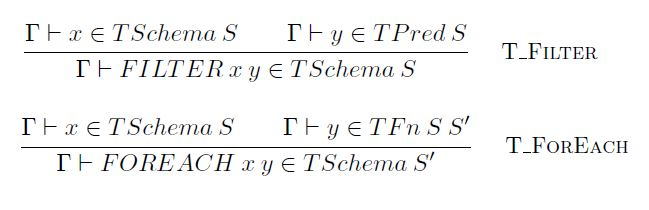
\includegraphics[width=1\linewidth]{Images/FilterForeach.JPG}
  \captionof{figure}{Typing Rules for FILTER and FOREACH}
  \label{fig:filter_foreach}
\end{figure}


\begin{figure}
\centering
  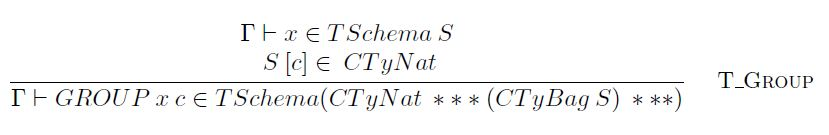
\includegraphics[width=1\linewidth]{Images/Group.JPG}
  \captionof{figure}{Typing Rule for Group}
  \label{fig:group}
\end{figure}

\begin{figure}
  \centering
  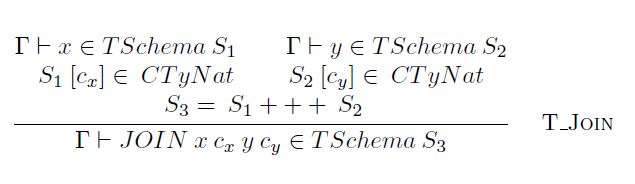
\includegraphics[width=1\linewidth]{Images/Join.JPG}
  \captionof{figure}{Typing Rule for Join}
  \label{fig:join}
\end{figure}

\begin{figure}
\centering
  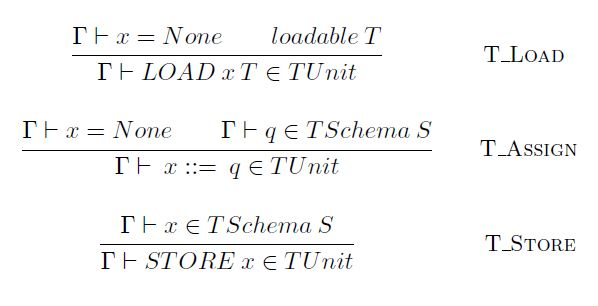
\includegraphics[width=1\linewidth]{Images/Load_Assign_Store.JPG}
  \captionof{figure}{Typing Rules for LOAD, ASSIGN and STORE}
  \label{fig:load_assign_store}
\end{figure}

\begin{figure}
\centering
  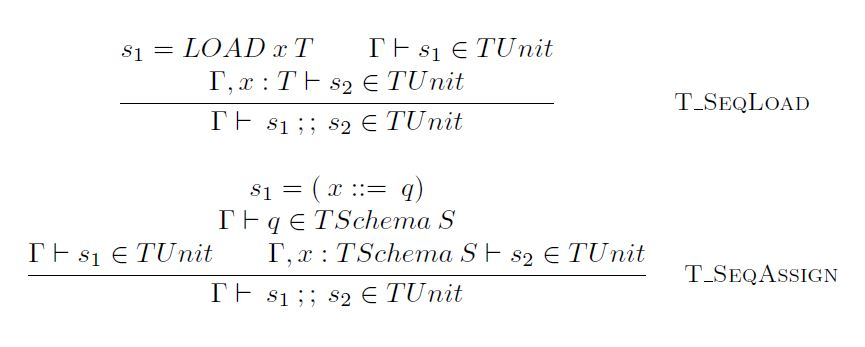
\includegraphics[width=1\linewidth]{Images/SEQ1.JPG}
  \captionof{figure}{Typing Rule for Sequence}
  \label{fig:seq1}
\end{figure}

\begin{figure}
  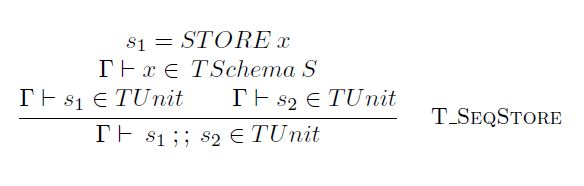
\includegraphics[width=1\linewidth]{Images/SEQ2.JPG}
  \captionof{figure}{Typing Rule for Sequence}
  \label{fig:seq2}
\end{figure}


{\bf TODO: present the new types, and the type rules here, and description of 
these rules that focuses on the new and interesting rules.}

